\subsection{元}
		集合の圏では集合から集合への関数の性質を述べるのに集合の元を用いることができるが、圏の対象では一般的に元を取ることができない。
		しかしある圏$\cat{C}$に\textbf{終対象}$1$と呼ばれる特別な対象が存在するとき、$\cat{C}$の任意の対象$A$のある\textbf{元(global elements)}はある射$\mor{a}{1}{A}$で表せる。
		\begin{center}
			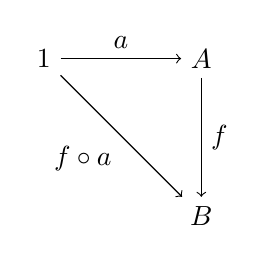
\begin{tikzpicture}[auto]
				\node (a) at (2, 0) {$A$};
				\node (b) at (2, -2) {$B$};
				\node (1) at (0, 0) {$1$};
				\draw[->] (1) to node {$a$}(a);
				\draw[->] (1) to node[swap] {$f\circ a$}(b);
				\draw[->] (a) to node {$f$}(b);
			\end{tikzpicture}
		\end{center}

		射$\mor{f}{A}{B}$に対して$\mor{a}{1}{A}$を適用する操作は、そのまま関数の合成$\mor{f\circ a}{1}{B}$で表せる。
		また射を適用した元もまた終対象からの射になるから$f\circ a$もまた対象$B$の元になる。

		後に詳しく説明するが、要素をただ一つ持つような集合は集合の圏における終対象$1$であり、$1$から集合$A$への写像である元は実際に集合$A$の元とみなせる。
		\begin{prop}[集合の圏における元]
			集合の圏には終対象となる集合$1$が存在し、任意の集合$A$において元$\mor{a}{1}{A}$は集合における元に対し一意に対応する。
		\end{prop}